\documentclass{bioinfo}
\copyrightyear{2005}
\pubyear{2005}

\begin{document}
\firstpage{1}

\title[bwa-meth]{Fast and accurate alignment of long bisulfite-seq reads}
\author[Pedersen \textit{et~al}]{
Brent S. Pedersen\,$^{1,}
\footnote{To whom correspondence should be addressed.  Email: bpederse@gmail.com}$,
Kenneth Eyring\,$^{1}$,
Subhajyoti De\,$^{1,2}$,
Ivana V. Yang\,$^{1}$
and David A. Schwartz\,$^1$%
}
\address{
    $^{1}$Department of Medicine, University of Colorado Denver, School of Medicine, Denver, Colorado, USA. 80045 \\
    $^{2}$University of Colorado Cancer Center, Molecular Oncology Program,
    Aurora, Colorado, USA
}

\history{Received on XXXXX; revised on XXXXX; accepted on XXXXX}

\editor{Associate Editor: XXXXXXX}

\maketitle

\begin{abstract}

    %http://www.oxfordjournals.org/our_journals/bioinformatics/for_authors/general.html

\section{Summary:}
We introduce a new tool, \textit{bwa-meth}, to align bisulfite-treated
sequences and compare it to existing aligners. We show that it is fast
and accurate even without quality-trimming and 
the output is immediately usable by downstream tools.
We gauge accuracy by comparing the number of on and off-target
reads from a targeted sequencing project and by simulations.

\section{Availability and Implementation:}
The benchmarking scripts and the \textit{bwa-meth} software are available at
https://github/com/brentp/bwa-meth/ under the MIT License.

\section{Contact:} \href{bpederse@gmail.com}{bpederse@gmail.com}
\section{Supplementary information:} 
Supplemental Information I
\end{abstract}

\section{Introduction}
Bisulfite sequencing (BS-Seq) is a common way to explore DNA methylation.
As a result, software 
has been developed to map sequence reads treated with bisulfite to a reference genome \citep{frithlast,methylcoder,gsnap,krueger2011,bsmap,bsmooth}.
Previous studies have compared alignment statistics on 
real \citep{methylcoder,bsmap,shrestha} and simulated \citep{frithlast} reads,
however most of these are limited by knowledge of the ground-truth and assumptions of
the simulation, respectively.

Here, we present an analysis of current BS-Seq mappers including the "four-base" aligners
Last \citep{frithlast}, GSNAP \citep{gsnap} and BSMAP \citep{bsmap} as well as the
"three-base" aligners BSmooth \citep{bsmooth}, Bison, and Bismark \citep{krueger2011} which
perform \emph{in silico} conversion of cytosines to thymines. In addtion, we introduce our
own, simple three-base aligner that wraps \textit{BWA mem} \citep{bwamem}.

The comparison is performed on 100-base paired-end reads
which are of modest length by current standards, but, to our knowledge, longer than
utilized in any comparison. We hypothesized that long, paired reads, with up
to 200 bases from the same genomic region, could change the decision on which
alignment method performed the best and that aligners which relied on global
alignment might have reduced performance on longer reads.
We found limitations to exisiting aligners including the writing of large temporary
files, required quality-trimming, high memory-use, long run-time, output that was not
suitable for consumption by traditional tools, or some combination of these
inconveniences. We wrote
a BS-Seq aligner based on BWA mem \citep{bwamem} to address these
limitations. This new aligner, 
\textit{bwa-meth}, allows indels, local alignments, and it never writes a
temporary-file of the reads to disk, instead streaming the \emph{in silico} converted
reads directly to the aligner and streaming the alignments directly to a well-formatted
alignment file suitable for use in downstream tools. In addition, it works well without
quality-trimming, thereby reducing storage requirements 3-fold by not creating
quality-trimmed or converted reads.

\section{Approach}
In order to determine the accuracy of an aligner,
we utilize a dataset from Agilent's SureSelect Mouse Methyl-Seq kit which
captures about
99 million bases from CpG dense regions in the mouse genome (a similar
approach is available for human regions).
We evaulate an aligner by the number of reads in the capture area as compared
to outside of the capture area. While there will be off-target capture, all
aligners are subject to the same assumptions. With those constraints, we can
plot a receiver operating curve (ROC) with true positives as reads within
and false positives as reads outside of the target regions.
\citealp{shrestha} performed an unbiased analysis on 35 base reads sequenced from
the X chromosome and called a read as accurately mapped if it aligned
to the X chromosome; here, we map to the entire genome with 100-base paired-end reads.

In addition, we map 100-base paired-end indel-free reads simulated using
Sherman (v0.1.6), the software from the authors of Bismark. All data were
aligned to mouse genome version \textit{mm10}.

\begin{methods}
\section{Methods}
We aligned real and simulated data, both as-is and trimmed by quality (using Trim Galore
[\href{http://www.bioinformatics.babraham.ac.uk/projects/trim\_galore/}{http://www.bioinformatics.babraham.ac.uk/projects/trim\_galore/}]
default parameters), using the software and versions in Supplemental Table 1.
We evaluated a few parameters for each method and report only the
best-performing here. Likely, every aligner could show improved results with
exhaustive search of the parameters, but this is a representation of
reasonable selections.
We considered a real read to be on-target if it was within 1001 bases
of a target region.

We designed \textit{bwa-meth} for paired-end reads from the directional
protocol but it can align single-end reads. \textit{bwa-meth} outputs alignments
directly to a BAM file that is usable even by those tools that require
coordinate-sorted alignments and read-groups. Since it consists
of fewer than 600 lines of code and runs
quickly, it can be used as a platform to test other optimizations. For example
in Supplemental Figure 7, we show a feature that further reduces the
number of off-target reads by considering only the single strand targeted by
the SureSelect protocol.

Although our comparisons are on an inbred mouse strain with few polymorphisms
we expect the results will hold even with insertions and deletions due to
our use of BWA mem \citep{bwamem}.

\end{methods}

\begin{figure}[!tpb]%figure1
    \centerline{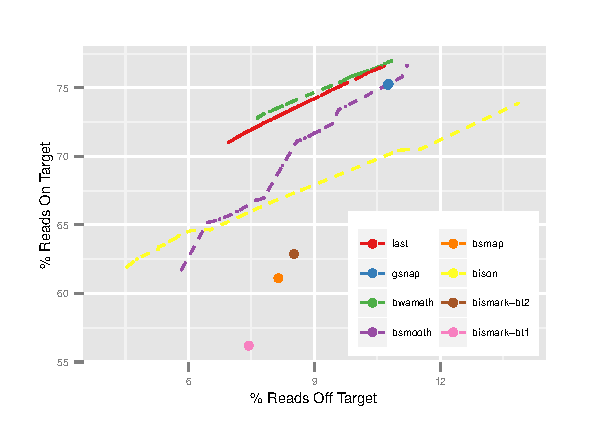
\includegraphics[width=86mm]{real-quals}}
    \caption{Percent of un-trimmed paired-end, 100-base reads on (y) and off (x)
    target for the tested aligners. Aligners that report mapping quality are
shown as connected dots for each quality cut-off. Reads are limited to those
considered as primary, mapped alignments by the aligner. Note that, as shown
in the supplement, many aligners have better performance on trimmed reads.
}\label{fig:01}
\end{figure}

\section{Discussion}

\subsection{Accuracy}
For the aligners that report a range of mapping quality
scores--an indicator of the aligner's confidence in the
alignment--we vary the score from 1 to the maximum, 255, to draw an ROC-like
curve showing the trade-off between sensitivity and specificity. For the
other aligners, we plot their single location. Figure \ref{fig:01} shows
the on and off-target reads for our real paired-end data. Last and 
\textit{bwa-meth} align the most reads on target with a low percent
of off-target reads, but Last can provide better control over the number
of off-target reads. On trimmed data, \textit{bwa-meth}, Last, Bison and
Bsmooth all perform similarly with Bison allowing very good control
over the number off-target reads (Supplement Figure 2).
Only Last, GSNAP, and \textit{bwa-meth} are relatively unaffected by quality-trimming.

Bismark performance varies depending on whether it uses bowtie version
1 or 2 for the backend but in either case, (as with all of the bowtie-backed
aligners) it performs better with trimmed reads.

A similar comparison is shown in Supplemental Figure 2 for trimmed data.
We also show the ROC figures for simulated data with errors in Supplemental
Figures 3 (original) and 4 (trimmed) and without errors in Supplemental 
Figures 5 and 6.
\textit{Bwa-meth} does out-perform all aligners for simulated data.

\subsection{Computational Resources}
We are more interested in the accuracy of a
method than the speed. In general the aligners are comparable in terms of
speed. While Bismark with bowtie1 is quite fast on the simulated data it
can not use multiple processes and so takes the longest user-time. Bsmap
takes the longest CPU time on the real data. We report the exact 
timings and maximum memory use in Supplemental Information.
Bsmap uses the least disk, never writing an index of the reference genome
and only writing the alignment files. All other aligners write an index of
the reference genome. Last, bsmooth, and bismark write additional copies of the
reads to disk.
\textit{Bwa-meth} avoids writing the \emph{in silico}
converted reads to disk by streaming them directly to the aligner and shows
nearly identical accuracy without read-trimming. The trimming and conversion
steps can increase data storage needs enough to be a burden in our experience. 

None of the programs used an inordinate amount of memory, however, due to
the parallelization strategy, Last did require about 10GB of shared memory
per process.

\section{Conclusion}
We have used simulated reads along with reads from a capture method that
targets CpG-rich regions to compare aligners.
We show that \textit{bwa-meth} is very accurate, even without quality trimming.
Aligners that use global alignment benefit more from quality trimming and may
also require an additional copy of the \emph{in silico} converted reads.
\textit{bwa-meth} is also fast and it outputs alignments to a sorted bam
that is immediately usable by downstream tools.

\section*{Acknowledgement}
We thank Devon Ryan for several helpful conversations.
\paragraph{Funding\textcolon} This was funded by R01 HL097163, R01 HL101251, 1I01BX001534, RC2 HL101715, N01 AI90052, and S10 RR031832.
%\bibliographystyle{natbib}
%\bibliographystyle{achemnat}
%\bibliographystyle{plainnat}
%\bibliographystyle{abbrv}
%\bibliographystyle{bioinformatics}
%
%\bibliographystyle{plain}
%
%\bibliography{Document}


%\begin{thebibliography}{}
\bibliographystyle{natbib}
    \bibliography{document}
%\end{thebibliography}
\end{document}
